\documentclass[a4paper,11pt,fleqn]{jarticle}
\usepackage[dvipdfmx]{graphicx}
\usepackage{float}
\usepackage{amsmath}
\usepackage{fancyhdr}

\def \vec#1{\mbox{\boldmath $#1$}} %ベクトルマクロ
\def \bun#1#2{\left(\frac{#1}{#2}\right)} %括弧つき分数マクロ
\def \rot{\nabla \times} %rot
\def \div{\nabla \cdot} %div
\def \intt{\int\!\!\!\int} %2重積分
\def \inttt{\int\!\!\!\int\!\!\!\int} %3重積分

% ページレイアウト
\setlength{\topmargin}{10mm}
  \addtolength{\topmargin}{-1in}
\setlength{\oddsidemargin}{30mm}
  \addtolength{\oddsidemargin}{-1in}
\setlength{\textwidth}{150mm}
\setlength{\textheight}{250mm}
\setlength{\headsep}{2zw}
\setlength{\headheight}{2zw}
\setlength{\topskip}{15mm}
\linespread{1.0}

% サブセクションを1.,2.にする設定
\renewcommand{\thesubsection}{\arabic{subsection}.}

% サブサブセクションを(1),(2)にする設定
\renewcommand{\thesubsubsection}{(\arabic{subsubsection})}

% 大問2の3番目の計算式のラベルを(2.3)にする設定
% 計算式の参照には\eqref{eq:hoge}を使う
\makeatletter
  \renewcommand{\theequation}{\arabic{subsection}.\arabic{equation}}
  \@addtoreset{equation}{subsection}
\pagestyle{fancy}
% ヘッダーの設定
  \lhead[物理数学 2016.05.02]{\leftmark}
  \rhead[\leftmark]{物理数学 2016.05.02}
\renewcommand{\headrulewidth}{0pt}
\makeatother



\begin{document}


\begin{center}
\begin{Large}
演習問題その9  常微分方程式(4) 解答例
\end{Large}
\end{center}

\subsection*{$※以下~x',\dot{x}=\frac{dx}{dt}~とする.$}
\subsection{$次の1階連立微分方程式を解け.$}
\subsubsection{}
$\left\{ \begin{array}{l}
x_1'=x_1+4x_2 \\
x_2'=2x_1+3x_2
\end{array} \right.$
\begin{eqnarray*}
(解答例)
\end{eqnarray*}
$D=\frac d{dt}$とおくと、与えられた方程式は
\[
\left\{
\begin{array}{rcl}
(D-1)x_1-4x_2 &=& 0 \\
-2x_1+(D-3)x_2 &=& 0
\end{array}
\right.
\]
と書き改められる。固有方程式
\[
\begin{array}{|cc|}
D-1 & -4 \\
-2 & D-3
\end{array}
=0
\]
を解くと、
\begin{eqnarray*}
(D-1)(D-3)-8&=&D^2-4D-5=(D+1)(D-5)=0 \\
\Leftrightarrow D &=& -1,5.
\end{eqnarray*}
よって$x_1=C_1e^{-t}+C_2e^{5t}$となる($C_1,C_2$は定数)。与えられた第1式より、
\begin{eqnarray*}
4x_2 &=& \frac{dx_1}{dt}-x_1 \\
&=& -C_1e^{-t}+5C_2e^{5t}-C_1e^{-t}-C_2e^{5t} \\
&=& -2C_1e^{-t}+4C_2e^{5t}.
\end{eqnarray*}
よって求める一般解は
\begin{eqnarray*}
\left\{ \begin{array}{rcl}
x_1&=&C_1e^{-t}+C_2e^{5t} \\
x_2&=&-\frac12C_1e^{-t}+C_2e^{5t}. \ \ \ \ 
\end{array}\right.
\end{eqnarray*}

\newpage
\subsubsection{}
$\left\{ \begin{array}{l}
x_1'=-x_1+2x_2 \\
x_2'=-2x_1-5x_2
\end{array} \right.$
\begin{eqnarray*}
(解答例)
\end{eqnarray*}
$D=\frac d{dt}$とおくと、与えられた方程式は
\[
\left\{
\begin{array}{rcl}
(D+1)x_1-2x_2 &=& 0 \\
2x_1+(D+5)x_2 &=& 0
\end{array}
\right.
\]
と書き改められる。固有方程式
\[
\begin{array}{|cc|}
D+1 & -2 \\
2 & D+5
\end{array}
=0
\]
を解くと、
\begin{eqnarray*}
(D+1)(D+5)-(-4)&=&D^2+6D+9=(D+3)^2=0 \\
\Leftrightarrow D &=& -3. \;\; (重解)
\end{eqnarray*}
よって$x_1=(C_1+C_2t)e^{-3t}$となる($C_1,C_2$は定数)。与えられた第1式より
\begin{eqnarray*}
2x_2 &=& \frac{dx_1}{dt}+x_1 \\
&=& C_2e^{-3t}-3(C_1+C_2t)e^{-3t}+(C_1+C_2t)e^{-3t} \\
&=& (C_2-2C_1-2C_2t)e^{-3t}.
\end{eqnarray*}
よって求める一般解は、
\begin{eqnarray*}
\left\{ \begin{array}{rcl}
x_1&=&(C_1+C_2t)e^{-3t} \\
x_2&=&\left(\frac12C_2-C_1-C_2t\right)e^{-3t}. \ \ \ \ 
\end{array}\right.
\end{eqnarray*}


\newpage
\subsubsection{}
$\left\{ \begin{array}{l}
x_1'=x_2+e^t \\
x_2'=x_1+e^{-t}
\end{array} \right.$
\begin{eqnarray*}
(解答例)
\end{eqnarray*}
\[
\left\{
\begin{array}{rcl}
x_1' &=& x_2 \\
x_2' &=& x_1
\end{array}
\right.
\]
の解は
\[
\left\{
\begin{array}{rcl}
x_1 &=& C_1'e^t+C_2'e^{-t} \\
x_2 &=& C_1'e^t-C_2'e^{-t}.
\end{array}
\right.
\]
$C_1'=z_1(t),C_2'=z_2(t)$とおいて元の方程式に代入すると、
\begin{eqnarray*}
\left\{
\begin{array}{rcl}
(z_1'+z_1)e^t+(z_2'-z_2)e^{-t} &=& z_1e^t-z_2e^{-t}+e^t \\
(z_1'+z_1)e^t+(-z_2'+z_2)e^{-t} &=& z_1e^t+z_2e^{-t}+e^{-t}
\end{array}
\right. \\
\Leftrightarrow \left\{
\begin{array}{rcl}
z_1'e^t+z_2'e^{-t} &=& e^t \\
z_1'e^t-z_2'e^{-t} &=& e^{-t}. \hspace{3cm}
\end{array}
\right.
\end{eqnarray*}
両辺の足し算から
\begin{eqnarray*}
z_1' &=& \frac{1+e^{-2t}}2. \\
積分して\ \ \ z_1 &=& \frac12t-\frac14e^{-2t}+C_1. \ \ \ \ \ (C_1は積分定数)
\end{eqnarray*}
両辺の引き算から
\begin{eqnarray*}
z_2' &=& \frac{e^{2t}-1}2. \\
積分して\ \ \ z_1 &=& \frac14e^{2t}-\frac12t+C_2. \ \ \ \ \ (C_2は積分定数)
\end{eqnarray*}
よって一般解は、
\begin{eqnarray*}
x_1 &=& \left(\frac12t-\frac14e^{-2t}+C_1\right)e^t+\left(\frac14e^{2t}-\frac12t+C_2\right)e^{-t} \\
&=& \left(\frac12t+\frac14\right)(e^t-e^{-t})+C_1e^t+C_2e^{-t} \\
x_2 &=& \left(\frac12t-\frac14e^{-2t}+C_1\right)e^t-\left(\frac14e^{2t}-\frac12t+C_2\right)e^{-t} \\
&=& \left(\frac12t-\frac14\right)(e^t+e^{-t})+C_1e^t-C_2e^{-t}.
\end{eqnarray*}


\newpage
\subsection{$次の3元連立微分方程式を解け.$}
\subsubsection{}
\begin{eqnarray*}
\left\{ \begin{array}{l}
x_{1}'=-x_{1}+x_{2}  \\
x_{2}'=-x_{2}+4x_{3} \\
x_{3}'=x_{1}-4x_{3}  
\end{array}\right.
\end{eqnarray*}
\begin{eqnarray*}
(解答例)
\end{eqnarray*}
$D=\frac d{dt}$とおくと、固有方程式は
\begin{eqnarray*}
\begin{array}{|ccc|}
D+1 & -1 & 0 \\
0 & D+1 & -4 \\
-1 & 0 & D+4
\end{array}
&=& 0 \\
\Leftrightarrow D(D+3)^2 &=& 0 \\
よって  x_1 &=& C_1e^{0t}+(C_2+C_3t)e^{-3t} \\
&=& C_1+(C_2+C_3t)e^{-3t}. \hspace{3cm}
\end{eqnarray*}
第1式より
\begin{eqnarray*}
x_2 &=& x_1'+x_1 \\
&=& C_3e^{-3t}-3(C_2+C_3t)e^{-3t}+C_1+(C_2+C_3t)e^{-3t} \\
&=& C_1+(-2C_2+C_3-2C_3t)e^{-3t}.
\end{eqnarray*}
第2式より
\begin{eqnarray*}
4x_3 &=& x_2'+x_2 \\
&=& (6C_2-3C_3+6C_3t-2C_3)e^{-3t}+C_1+(-2C_2+C_3-2C_3t)e^{-3t} \\
&=& C_1+(4C_2-4C_3+4C_3t)e^{-3t} \\
x_3 &=& \frac14C_1+(C_2-C_3+C_3t)e^{-3t}.
\end{eqnarray*}
よって一般解は、$\frac14C_1$を$C_1$と書き直して、
\begin{eqnarray*}
\left\{ \begin{array}{rcl}
x_1&=&4C_1+(C_2+C_3t)e^{-3t} \\
x_2&=&4C_1+(-2C_2+C_3-2C_3t)e^{-3t} \ \\
x_3&=&C_1+(C_2-C_3+C_3t)e^{-3t}. \ 
\end{array}\right.
\end{eqnarray*}

\newpage
\subsection{$aを定数とする.連立微分方程式~\frac{dx}{dt}+ay=0,~ax-\frac{dy}{dt}=0~を解け.また、その解(x,y)はどんな図形を描くか.$}
\begin{eqnarray*}
(解答例)
\end{eqnarray*}
\begin{enumerate}
\item $a=0$のとき\\
$\dot{x}=0,~\dot{y}=0$なので、$x=c_1,~x=c_2(ただし、c_1,c_2は定数)$\\
よって、$(x,y)$は1点$(c_1,c_2)$を描く.
\item $a\neq 0$のとき\\
$y=-\frac{1}{a}\dot{x}$なので、$\dot{y}=-\frac{1}{a}\ddot{x}$\\
よって、$\ddot{x}+a^2x=0$が導かれる.\\
$x=e^{\lambda t}$とおいて、固有方程式${\lambda}^2+a^2=0$を解くと、\\
$\lambda =\pm ai$\\
よって、$x=c_1\cos at+c_2\sin at(ただし、c_1,c_2は定数)$\\
$y=-\frac{1}{a}\dot{x}=c_1\sin at-c_2\cos at$\\
このとき、$x^2+y^2=c_1^2+c_2^2=const.$\\
よって$(x,y)$は円を描く.
\end{enumerate}


\newpage
\subsection{}
等質量$m$のおもり1,2がバネにつながれている.各バネのバネ定数は全て同じ$k$である.以下の問いに答えよ.
\begin{figure}[htpb]
\begin{center}
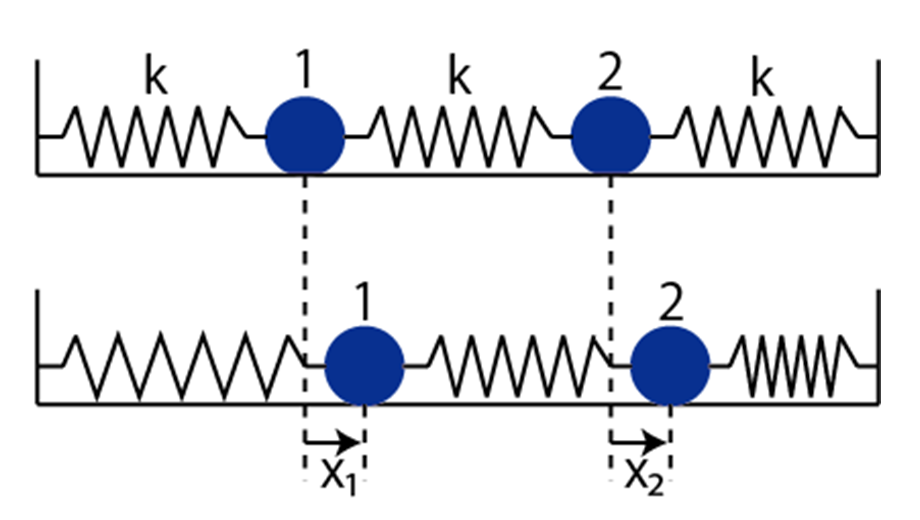
\includegraphics[scale=.25]{bane.png}
\end{center}
\end{figure}
\subsubsection{$おもり1,2それぞれの平衡点からの変位をx_1,x_2としておもりの運動方程式を求めよ.$}
(解答例)\\
\\
$\left\{ \begin{array}{l}
m\ddot{x_1}=-kx_1-k(x_1-x_2)=-2kx_1+kx_2 \\
m\ddot{x_2}=-kx_2+k(x_1-x_2)=kx_1-2kx_2
\end{array} \right.$
\subsubsection{$x_1,x_2の一般解を求めよ.$}
(解答例)\\
連立している式の和と差をとることにより、\\
\\
$\left\{ \begin{array}{l}
m(\ddot{x_1}+\ddot{x_2})=-k(x_1+x_2) \\
m(\ddot{x_1}-\ddot{x_2})=-3k(x_1-x_2)
\end{array} \right.$\\
よって、\\
$\left\{ \begin{array}{l}
x_1+x_2=a\cos({\omega}_1t+\alpha),\quad {\omega}_1=\sqrt{k/m} \\
x_1-x_2=b\cos({\omega}_2t+\beta),\quad {\omega}_2=\sqrt{3k/m}
\end{array} \right.$\\
$(ただし、a,b,\alpha ,\beta は定数)$\\
\\
したがって一般解は、
\begin{eqnarray*}
x_1=\frac{1}{2}a\cos({\omega}_1t+\alpha)+\frac{1}{2}b\cos({\omega}_2t+\beta)
\end{eqnarray*}
\begin{eqnarray*}
x_2=\frac{1}{2}a\cos({\omega}_1t+\alpha)-\frac{1}{2}b\cos({\omega}_2t+\beta)
\end{eqnarray*}

\newpage
\section*{$+\alpha 問題$}
\subsection{$次の1階連立微分方程式を解け.$}
\subsubsection{}
$\left\{ \begin{array}{l}
x'=-x+2y+\cos t\qquad \cdots (i) \\
y'=2x-y \qquad \cdots (ii)
\end{array} \right.$\\
\\
(解答例)\\
(i)+(ii)より、$x+y=X$とおいて、
\begin{eqnarray*}
X'=X+\cos t \qquad \cdots (i)'
\end{eqnarray*}
(i)-(ii)より、$x-y=Y$とおいて、
\begin{eqnarray*}
Y'=-3Y+\cos t \qquad \cdots (ii)'
\end{eqnarray*}
(i)'の斉次解は、$X'=X$を解いて、$X=c_1e^t(ただし、c_1は定数)$.\\
特殊解を$A\cos t+B\sin t$とおくと、\\
$-A\sin t+B\cos t=A\cos t+B\sin t+\cos t$\\
これを解いて、$A=-1/2,~B=1/2$\\
よって(i)'の一般解は、
\begin{eqnarray*}
X=c_1e^t-\frac{1}{2}\cos t+\frac{1}{2}\sin t
\end{eqnarray*}
(ii)'についても同様にして、
\begin{eqnarray*}
Y=c_2e^{-3t}+\frac{3}{10}\cos t+\frac{1}{10}\sin t\qquad (ただしc_2は定数)
\end{eqnarray*}
よって、
\begin{eqnarray*}
x=\frac{X+Y}{2}=\frac{c_1}{2}e^t+\frac{c_2}{2}e^{-3t}-\frac{1}{10}\cos t+\frac{3}{10}\sin t
\end{eqnarray*}
\begin{eqnarray*}
y=\frac{X-Y}{2}=\frac{c_1}{2}e^t-\frac{c_2}{2}e^{-3t}-\frac{2}{5}\cos t+\frac{1}{5}\sin t
\end{eqnarray*}

\newpage
\subsubsection{}
$\left\{ \begin{array}{l}
{x'}_1=-x_2+\sin t \\
{x'}_2= x_1+\cos t
\end{array} \right.$
\begin{eqnarray*}
(解答例)
\end{eqnarray*}
\[
\left\{
\begin{array}{rcl}
x_1' &=& -x_2 \\
x_2' &=& x_1
\end{array}
\right.
\]
の解は
\[
\left\{
\begin{array}{rcl}
x_1 &=& C_1'\cos t+C_2'\sin t \\
x_2 &=& C_1'\sin t-C_2'\cos t.
\end{array}
\right.
\]
$C_1'=z_1(t),C_2'=z_2(t)$とおいて元の方程式に代入すると
\[
\left\{
\begin{array}{rcl}
z_1'\cos t+z_2'\sin t-z_1\sin t+z_2\cos t &=& -(z_1\sin t-z_2\cos t)+\sin t \\
z_1'\sin t-z_2'\cos t+z_1\cos t+z_2\sin t &=& z_1\cos t+z_2\sin t+\cos t
\end{array}
\right. 
\]
\begin{eqnarray}
\Leftrightarrow
z_1'\cos t+z_2'\sin t &=& \sin t
\label{1} \\
z_1'\sin t-z_2'\cos t &=& \cos t. \label{2} 
\end{eqnarray}
(1)式$\times \cos t+$(2)式$\times \sin t$より
\begin{eqnarray*}
z_1' &=& 2\sin t\cos t=\sin2t. \\
積分して \hspace{2cm} z_1 &=& -\frac{\cos2t}2+C_1. \ \ \ \ (C_1は積分定数)
\end{eqnarray*}
(1)式$\times \sin t-$(2)式$\times \cos t$より
\begin{eqnarray*}
z_2' &=& \sin^2t-\cos^2 t=-\cos2t. \\
積分して \hspace{2cm} z_2 &=& -\frac{\sin2t}2+C_2. \ \ \ \ (C_2は積分定数)
\end{eqnarray*}
よって一般解は、
\begin{eqnarray*}
x_1 &=& \left(-\frac{\cos2t}2+C_1\right)\cos t+\left(-\frac{\sin2t}2+C_2\right)\sin t \\
&=& C_1\cos t+C_2\sin t-\frac12\cos t \; \; \; (\cos2t\cos t+\sin2t\sin t=\cos(2t-t)\ より) \\
x_2 &=& \left(-\frac{\cos2t}2+C_1\right)\sin t-\left(-\frac{\sin2t}2+C_2\right)\cos t \\
&=& C_1\sin t-C_2\cos t+\frac12\sin t \ \ \ ( \sin2t\cos t-\cos2t\sin t=\sin(2t-t)\ より).
\end{eqnarray*}


\newpage
\subsection{}
\subsubsection{$以下の連立微分方程式を解け.ただし\Omega ,\eta は定数とする.$}
$\left\{ \begin{array}{l}
\ddot{x}-2\Omega \dot{y}=-\eta x \qquad \cdots (i) \\
\ddot{y}+2\Omega \dot{x}=0 \qquad \cdots (ii)
\end{array} \right.$
\\
\\
(解答例)\\
(i)の両辺を時間微分すると、$x'''-2\Omega y''=-\eta x'$\\
(ii)を代入して、\\
$x'''+4{\Omega}^2=-\eta x'$\\
$x'''=-(4{\Omega}^2+\eta)x'$\\
よって、$x'=A\cos(kt+\alpha) \qquad (ただしk^2=4{\Omega}^2+\eta ~,Aと\alpha は定数)$\\
これを積分して、
\begin{eqnarray*}
x=\frac{A}{k}\sin(kt+\alpha)+c_1 \qquad (c_1は定数)
\end{eqnarray*}
(ii)に代入して、\\
$y''=-2A\Omega\cos(kt+\alpha)$\\
よって、
\begin{eqnarray*}
y=\frac{2A\Omega}{k^2}\cos(kt+\alpha)
\end{eqnarray*}
これらを(i)に代入すると$c_1=0$となるので、一般解は、
\begin{eqnarray*}
x=\frac{A}{k}\sin(kt+\alpha)
\end{eqnarray*}
\begin{eqnarray*}
y=\frac{2A\Omega}{k^2}\cos(kt+\alpha)
\end{eqnarray*}
\begin{figure}[htpb]
\begin{center}
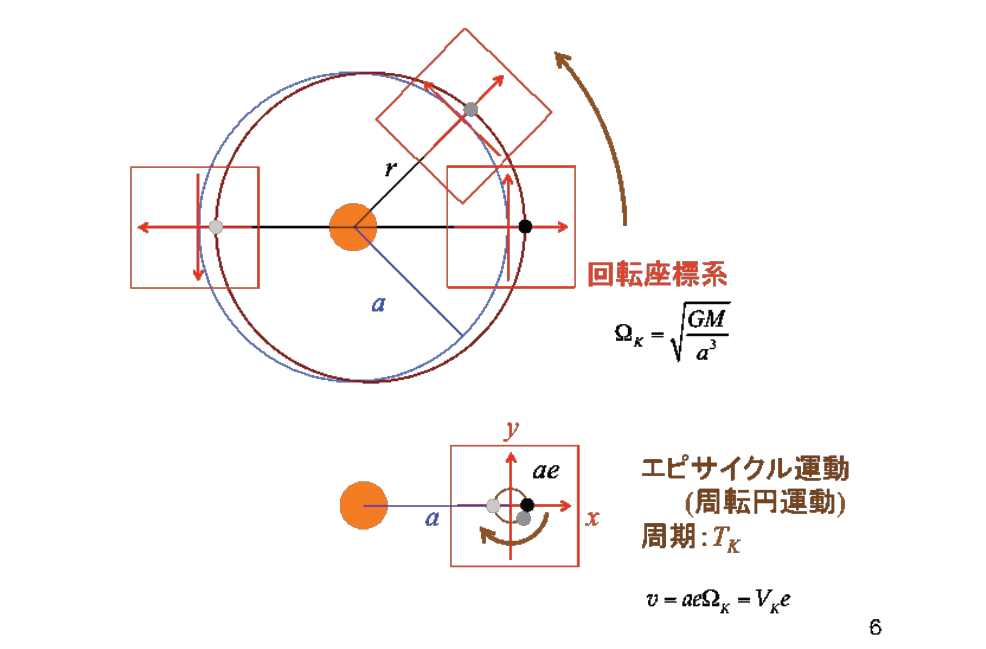
\includegraphics[scale=.30]{nakamoto.png}
\end{center}
\end{figure}
[補足]\\
図は、同じ軌道長半径を持った円運動と楕円運動を、重心を一点に固定して重ねたものである(中本2012,惑星科学フロンティアセミナー講演資料より引用)。円軌道上を回転する座標系から楕円軌道を描く粒子の運動を見ると、この楕円運動は「エピサイクル運動(周転円運動)」をしているように見えることが分かる。ここで求めた解は、このようなエピサイクル運動を表している。

\newpage
\subsection{}
等質量$m$のおもり1,2がバネにつながれている.各バネのバネ定数は図の通り(順に$k,K,k$)である.このとき、おもり1,2のそれぞれの変位を$x_1,x_2$としてそれぞれのおもりの運動方程式は、
\begin{eqnarray*}
\left\{
\begin{array}{l}
m\ddot{x}_1 = -kx_1 + K(x_2-x_1), \\
m\ddot{x}_2 = -kx_2 - K(x_2-x_1),
\end{array}
\right.
\end{eqnarray*}
となる.
初期条件として、おもり1,2の速度をそれぞれ$\dot{x}_1 = 2\sqrt{(k + K)/m},\ \dot{x}_2 = -2\sqrt{K/m}$としたときの
$x_1(t),~x_2(t)$を求めよ.
\begin{figure}[htpb]
\begin{center}
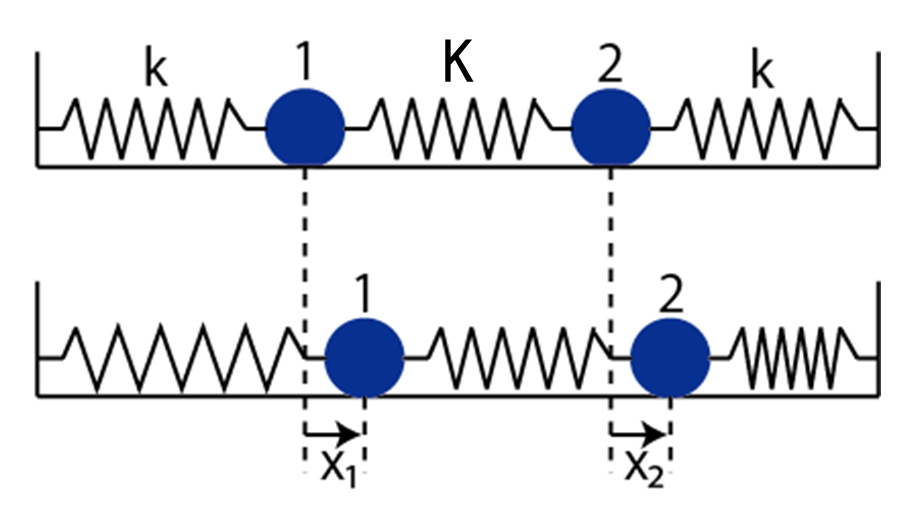
\includegraphics[scale=.25]{bane2.png}
\end{center}
\end{figure}
\begin{eqnarray*}
(解答例)
\end{eqnarray*}
$D=\frac d{dt}$とおくと$D^2=\frac{d^2}{dt^2}$となり、与えられた方程式は
\[
\left\{
\begin{array}{rcl}
(mD^2+k+K)x_1 - Kx_2&=& 0 \\
-Kx_1 + (mD^2+k+K)x_2 &=& 0.
\end{array}
\right.
\]
と書き改められる。固有方程式
\[
\begin{array}{|cc|}
(mD^2+k+K) & -K \\
-K & (mD^2+k+K)
\end{array}
=0
\]
を解くと、
\begin{eqnarray*}
&&m^2D^4 + 2m{k+K}D^2 + (k^2 + 2Kk)=0, \\
&&\Leftrightarrow D^2 = -\frac{k}{m},-\frac{k+2K}{m}\ \Leftrightarrow D = \pm\sqrt{\frac{k}{m}}i,\ \pm\sqrt{\frac{k+2K}{m}}i.
\end{eqnarray*}
よって
\begin{eqnarray*}
x_1=C_1\cos\sqrt{\frac{k}{m}}t+C_2\sin\sqrt{\frac{k}{m}}t+C_3\cos\sqrt{\frac{k+2K}{m}}t+C_4\sin\sqrt{\frac{k+2K}{m}}t.
\end{eqnarray*}
ここまでが一般解である。

以下、初期条件を考慮して$C_1,C_2,C_3,C_4$を求めていく。\\
$t=0$で変位$x_1 = 0$となるので、$C_1 = C_3 = 0$。よって
\[
x_1=C_2\sin\sqrt{\frac{k}{m}}t+C_4\sin\sqrt{\frac{k+2K}{m}}t.
\]
おもり1に関する運動方程式に代入すれば、
\[
x_2=C_2\sin\sqrt{\frac{k}{m}}t-C_4\sin\sqrt{\frac{k+2K}{m}}t.
\]
また、$x_1,x_2$を$t$で1回微分すれば、

\[
\left\{
\begin{array}{rcl}
\dot{x}_1 &=& \sqrt{\frac{k}{m}}C_2\cos\sqrt{\frac{k}{m}}t + \sqrt{\frac{k+2K}{m}}C_4\cos\sqrt{\frac{k+2K}{m}}t\\
\dot{x}_2 &=& \sqrt{\frac{k}{m}}C_2\cos\sqrt{\frac{k}{m}}t - \sqrt{\frac{k+2K}{m}}C_4\cos\sqrt{\frac{k+2K}{m}}t.
\end{array}
\right.
\]

$t=0$における初期速度を代入すれば、
\[
\left\{
\begin{array}{rcl}
2\sqrt{\frac{k+K}{m}} &=& \sqrt{\frac{k}{m}}C_2 + \sqrt{\frac{k+2K}{m}}C_4\\
-2\sqrt{\frac{K}{m}} &=& \sqrt{\frac{k}{m}}C_2 - \sqrt{\frac{k+2K}{m}}C_4.
\end{array}
\right.
\]
よって$C_2 = C_4 = 1$。以上より変位$x_1,\ x_2$は、
\[
\left\{
\begin{array}{rcl}
x_1 &=& \sin\sqrt{\frac{k}{m}}t+\sin\sqrt{\frac{k+2K}{m}}t\\
x_2 &=& \sin\sqrt{\frac{k}{m}}t-\sin\sqrt{\frac{k+2K}{m}}t.
\end{array}
\right.
\]


\newpage
\subsection{$動物生態学では、カナダオオヤマネコの個体数と野ウサギの個体数が10年程度の時間で振動することが知られている。以下、このダイナミクスを簡単なモデルで数理化することを考える。$}
被食者(野ウサギ)の個体数を$X$、捕食者(カナダオオヤマネコ)の個体数を$Y$とおく。ここで個体数は実数で近似する。
被食者は草食動物で、自然出生率に応じて$\frac{dX}{dt}=AX$にて指数関数的に増殖する。ただし捕食者があると、その数に比例して食われるために、個体数変化には$-BXY$の減少効果が見込まれる。\par
一方、捕食者$Y$の増加率は被食者数に比例する$\frac{dY}{dt}=CXY$と考えられるが、被食者がいなければ自然減少するので、個体数変化には$-DY$の減少効果が含まれる。これらの効果を総合することによって、以下の非線形連立微分方程式が得られる;\\
\\
$\left\{ \begin{array}{l}
\dot{X}=(A-BY)X \qquad \cdots (i) \\
\dot{Y}=(CX-D)Y \qquad \cdots (ii)
\end{array} \right.$
\\
\\
この方程式はロトカ=ヴォルテラ方程式と呼ばれ、振動解を持つことが知られている。\\
以下の問いに答えよ。

\subsubsection{$この方程式は非線形(XYの項を含む)なので、解析的に解くことが難しい。そこでここでは簡単のため、\dot{X}=\dot{Y}=0を満たす不動点(X,Y)=(D/C,A/B)からのずれ(x,y)=(X-D/C,Y-A/B)を考えることにする。|x|,|y|が小さいとして\mathcal{O}(xy)の項を無視することにより、以下の線形連立微分方程式を導出せよ。$}
$\left\{ \begin{array}{l}
\dot{x}=-\frac{BD}{C}y \qquad \cdots (i)' \\
\dot{y}=\frac{CA}{B}x \qquad \cdots (ii)'
\end{array} \right.$\\
\\
(解答例)\\
$X=x+\frac{D}{C},~Y=y+\frac{A}{B}$であるので、まずこれを(i)に代入して、
\begin{eqnarray*}
\frac{d}{dt}\left(x+\frac{D}{C}\right)=-By\cdot\left(x+\frac{D}{C}\right)
\end{eqnarray*}
\begin{eqnarray*}
\dot{x}=-By\cdot\left(x+\frac{D}{C}\right)
\end{eqnarray*}
(ii)にも代入し、同様にして、
\begin{eqnarray*}
\dot{y}=Cx\cdot\left(y+\frac{A}{B}\right)
\end{eqnarray*}
ここで、$x,y$を微小とみなし$xy$の項を無視することで、与式が得られる。

\newpage
\subsubsection{}
$x,y$に関する(1)の微分方程式を解くことによって、$y$が$x$の振動に$\pi /2$だけ遅れて追従することを示せ。\\
\\
(解答例)\\
(i)'を時間微分して、$\ddot{x}=-\frac{BD}{C}\dot{y}$\\
これに(ii)'を代入すると、
\begin{eqnarray*}
\ddot{x}=-\frac{BD}{C}\cdot\frac{AC}{B}x
\end{eqnarray*}
\begin{eqnarray*}
\ddot{x}=-ADx
\end{eqnarray*}
${\omega}^2=AD$とおくと、
\begin{eqnarray*}
\ddot{x}+{\omega}^2x=0
\end{eqnarray*}
これは調和振動の式であり、被食者の個体数ゆらぎ$x$は$\omega =\sqrt{AD}$で振動することが分かる。\\
捕食者の個体数ゆらぎ$y$は、(i)'により、
\begin{eqnarray*}
y=-\frac{C}{BD}\dot{x}
\end{eqnarray*}
で与えられるので、$y$も$x$の振動に伴って同じ周期で振動することが分かる。被食者の振動を$x\propto\cos(\omega t)$とおいて(i)'に代入すると、
\begin{eqnarray*}
y\propto\sin(\omega t)=\cos\left(\omega t-\frac{\pi}{2}\right)
\end{eqnarray*}
このことから、$y$は$x$の振動に$\pi /2$遅れて追従することが分かる。これは「被食者数$X$が増えればそれを受けて捕食者数$Y$が増大し、被食者数が減ればそれに伴って捕食者数も減少する」という状況を表している。\\
図はロトカ=ヴォルテラ方程式の解の一例である。横軸は時間で縦軸は個体数であり、このように、被食者と捕食者の個体数変動の位相がずれている。
\begin{figure}[htpb]
\begin{center}
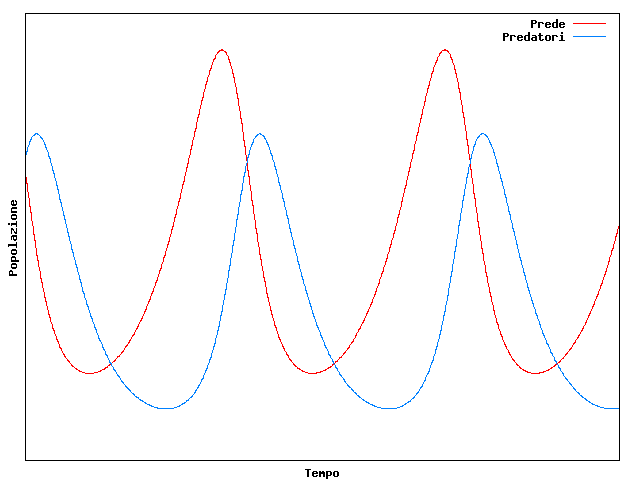
\includegraphics[scale=.30]{Lotka-Volterra.png}
\end{center}
\end{figure}

\end{document}